% !TEX program = xelatex

% Base
\documentclass{article}
\usepackage[a4paper,margin=1in]{geometry}

% Locale
\usepackage{polyglossia}
\setdefaultlanguage[localalph=true]{slovenian}
\usepackage[autostyle]{csquotes}
\DeclareQuoteAlias{german}{slovene}

% Bibliography
\usepackage[backend=biber,style=numeric]{biblatex}
\addbibresource{/home/martin/literatura.bib}

% Math
\usepackage{amsmath}
\usepackage{amssymb}
\usepackage{siunitx}

% Imported pdf_tex figures
\usepackage{graphicx,import}
\usepackage{subfig}
\usepackage{color}

% Hyperlinks
\usepackage{hyperref}
\usepackage[svgnames]{xcolor}

% Pgfplots
\usepackage{amssymb}

% Styling
\numberwithin{equation}{section}
\setlength{\skip\footins}{1.5cm}

% Differential
\newcommand{\diff}{\mathrm{d}}

% "Defined as" symbol
\usepackage{mathtools}
\newcommand{\das}{\vcentcolon=}
\newcommand{\asd}{=\vcentcolon}

\title{Difuzija tekočin}

\author{Martin Šifrar}

\begin{document}

\maketitle

\section{Uvod}

\subsection{Lom}

Če pri lomu žarka na eni meji sredstva velja med kotoma, ki ga žarek objema z optično osjo zveza

\begin{equation*}
    \frac{\cos \varphi_1}{\cos \varphi_2} = \frac{n_2}{n_1},
\end{equation*}

pri čemer sta $n_1$ in $n_2$ lomna količnika. Če ta produkt zapišemo za $N$ plasti, lahko z logaritmiranjem produkt prevedemo na vsoto. Ko $N$ pošljemo proti neskončno, dobimo zvezo

\begin{equation}
    \diff(\log \cos\varphi) = -\diff(\log n).
    \label{eq:d-snell}
\end{equation}

\begin{figure}
    \begin{center}
        \includegraphics[width=0.8\textwidth]{diagram.png}
    \end{center}
    \caption{Lom žarka znotraj sredstva (levo) in pot žarka skozi kiveto proti zaslonu (desno).}
    \label{fig:diagram}
\end{figure}

V našem primeru je lomni količnik odvisen le od koordinate $z$. Torej lahko izraz~(\ref{eq:d-snell}) integriramo po $x$. Z dodatnim upoštevanjem meje na robu kivete (glej sliko~\ref{fig:diagram}) dobimo

\begin{equation*}
    \alpha_Z = d \frac{\diff n}{\diff z}.
\end{equation*}

To se na zaslonu pokaže kot odmik $h$, ki je za majhne kote $\alpha$ in $d \ll b$ enak

\begin{equation}
    y(z) = bd \frac{\diff n}{\diff z}.
    \label{eq:y}
\end{equation}

\subsection{Difuzija}

V kiveti za koncentracijo etanola $f(z)$ velja eno-dimenzionalna difuzijska enačba

\begin{equation*}
    \left[ \frac{\partial^2}{\partial z^2} - \frac{1}{D} \frac{\partial}{\partial t} \right] f = 0
\end{equation*}

Osnovna rešitev te enačbe je $f = \frac{1}{\sqrt{4\pi Dt}} e^{-\frac{z^2}{4Dt}}$, kar predstavlja rešitev za začetno koncentracijo $f \propto \delta(z)$. Če z integriranjem te Greenove formule enčbe rešimo pri naših začetnih pogojih, dobimo odvisnost lomnega količnika, ki ga narekuje mešanje vode z količnikom $n_0$ in etanola z lomnim količnikom $n_1$

\begin{equation*}
    n(z) = \frac{n_0 + n_1}{2} + \frac{n_1 - n_0}{2} \theta \left( \frac{z}{\sqrt{4Dt}} \right).
\end{equation*}

Če to vstavimo v enačbo~(\ref{eq:y}), dobimo odmik na zaslonu

\begin{equation*}
    y(z) = bd(n_1 - n_0) \frac{1}{\sqrt{4\pi Dt}} e^{-\frac{z^2}{4Dt}}.
\end{equation*}

Ploščina pod to krivuljo je konstantna s časom in je enaka

\begin{equation}
    S = kbd(n_1 - n_0),
    \label{eq:S}
\end{equation}

pri čemer je $k = \frac{a+b}{a}$, a pa razdalja med stekleno paličico in kiveto. Maksimalen odmik $y$ je sorazmeren z $1/\sqrt{t}$

\begin{equation}
    h = \frac{bd(n_1 - n_0)}{\sqrt{4\pi Dt}}.
    \label{eq:h}
\end{equation}

\section{Naloga}

\begin{enumerate}
    \item Izmeri časovno odvisnost maksimalne višine $h$, krivulje na zaslonu nad diagonalo.
    \item Iz enačbe~(\ref{eq:h}) izrazi $Dt$ in s prilagajanjem premice izračunaj difuzijsko konstanto $D$.
\end{enumerate}

\section{Meritve}

Prvo izmerimo razdaljo med stekleno paličico (s katero razpršimo snop) in kiveto, debelino kivete in razdaljo med kiveto in zalonom

\begin{align*}
    a &= (49 \pm 1)\,\mathrm{cm}, \\
    d &= (12 \pm 1)\,\mathrm{mm}, \\
    b &= (87 \pm 1)\,\mathrm{cm}.
\end{align*}

V kiveto nalijemo etanol, nato pa na dno z cevko previdno nalijemo destilirano vodo. Začnemo štoparico in na zaslonu na milimeterski papir beležimo maksimalne odmike~(glej sliki~\ref{fig:ticks}~in~\ref{fig:by-t})

\begin{figure}
    \begin{center}
        \includegraphics{by-t.pdf}
    \end{center}
    \caption{Potek maksimalnega odmika $h$ po času.}
    \label{fig:by-t}
\end{figure}

Ob treh različnih časih orišemo tudi obliko krivulje. Njeno površino izračunamo tako, da jo orišemo s trikotniki~(slika~\ref{fig:meas}). Izračunane površine so

\begin{align*}
    S_1 &= 1392\,\mathrm{mm^2}, \\
    S_2 &= 1395\,\mathrm{mm^2}, \\
    S_3 &= 1395\,\mathrm{mm^2}.
\end{align*}

V našem modelu je površina konstantna, torej lahko iz treh meritev dobimo povprečno vrednost in oceno napake

\begin{equation*}
    S = (1394 \pm 1)\,\mathrm{mm^2}.
\end{equation*}

To se ujema s površino, ki jo predvideva enačba~(\ref{eq:S})

\begin{equation*}
    S_\mathrm{predvidena} = (1330 \pm 90)\,\mathrm{mm^2}
\end{equation*}

\begin{figure}
    \begin{center}
        \includegraphics[width=0.6\textwidth]{ticks.jpg}
    \end{center}
    \caption{Zaslon, na katerega beležimo maksimalen odmik $h$ ob različnih časih. Dodatno so na papir orisane oblike krivulje ob treh različnih časih.}
    \label{fig:ticks}
\end{figure}

\begin{figure}
    \begin{center}
        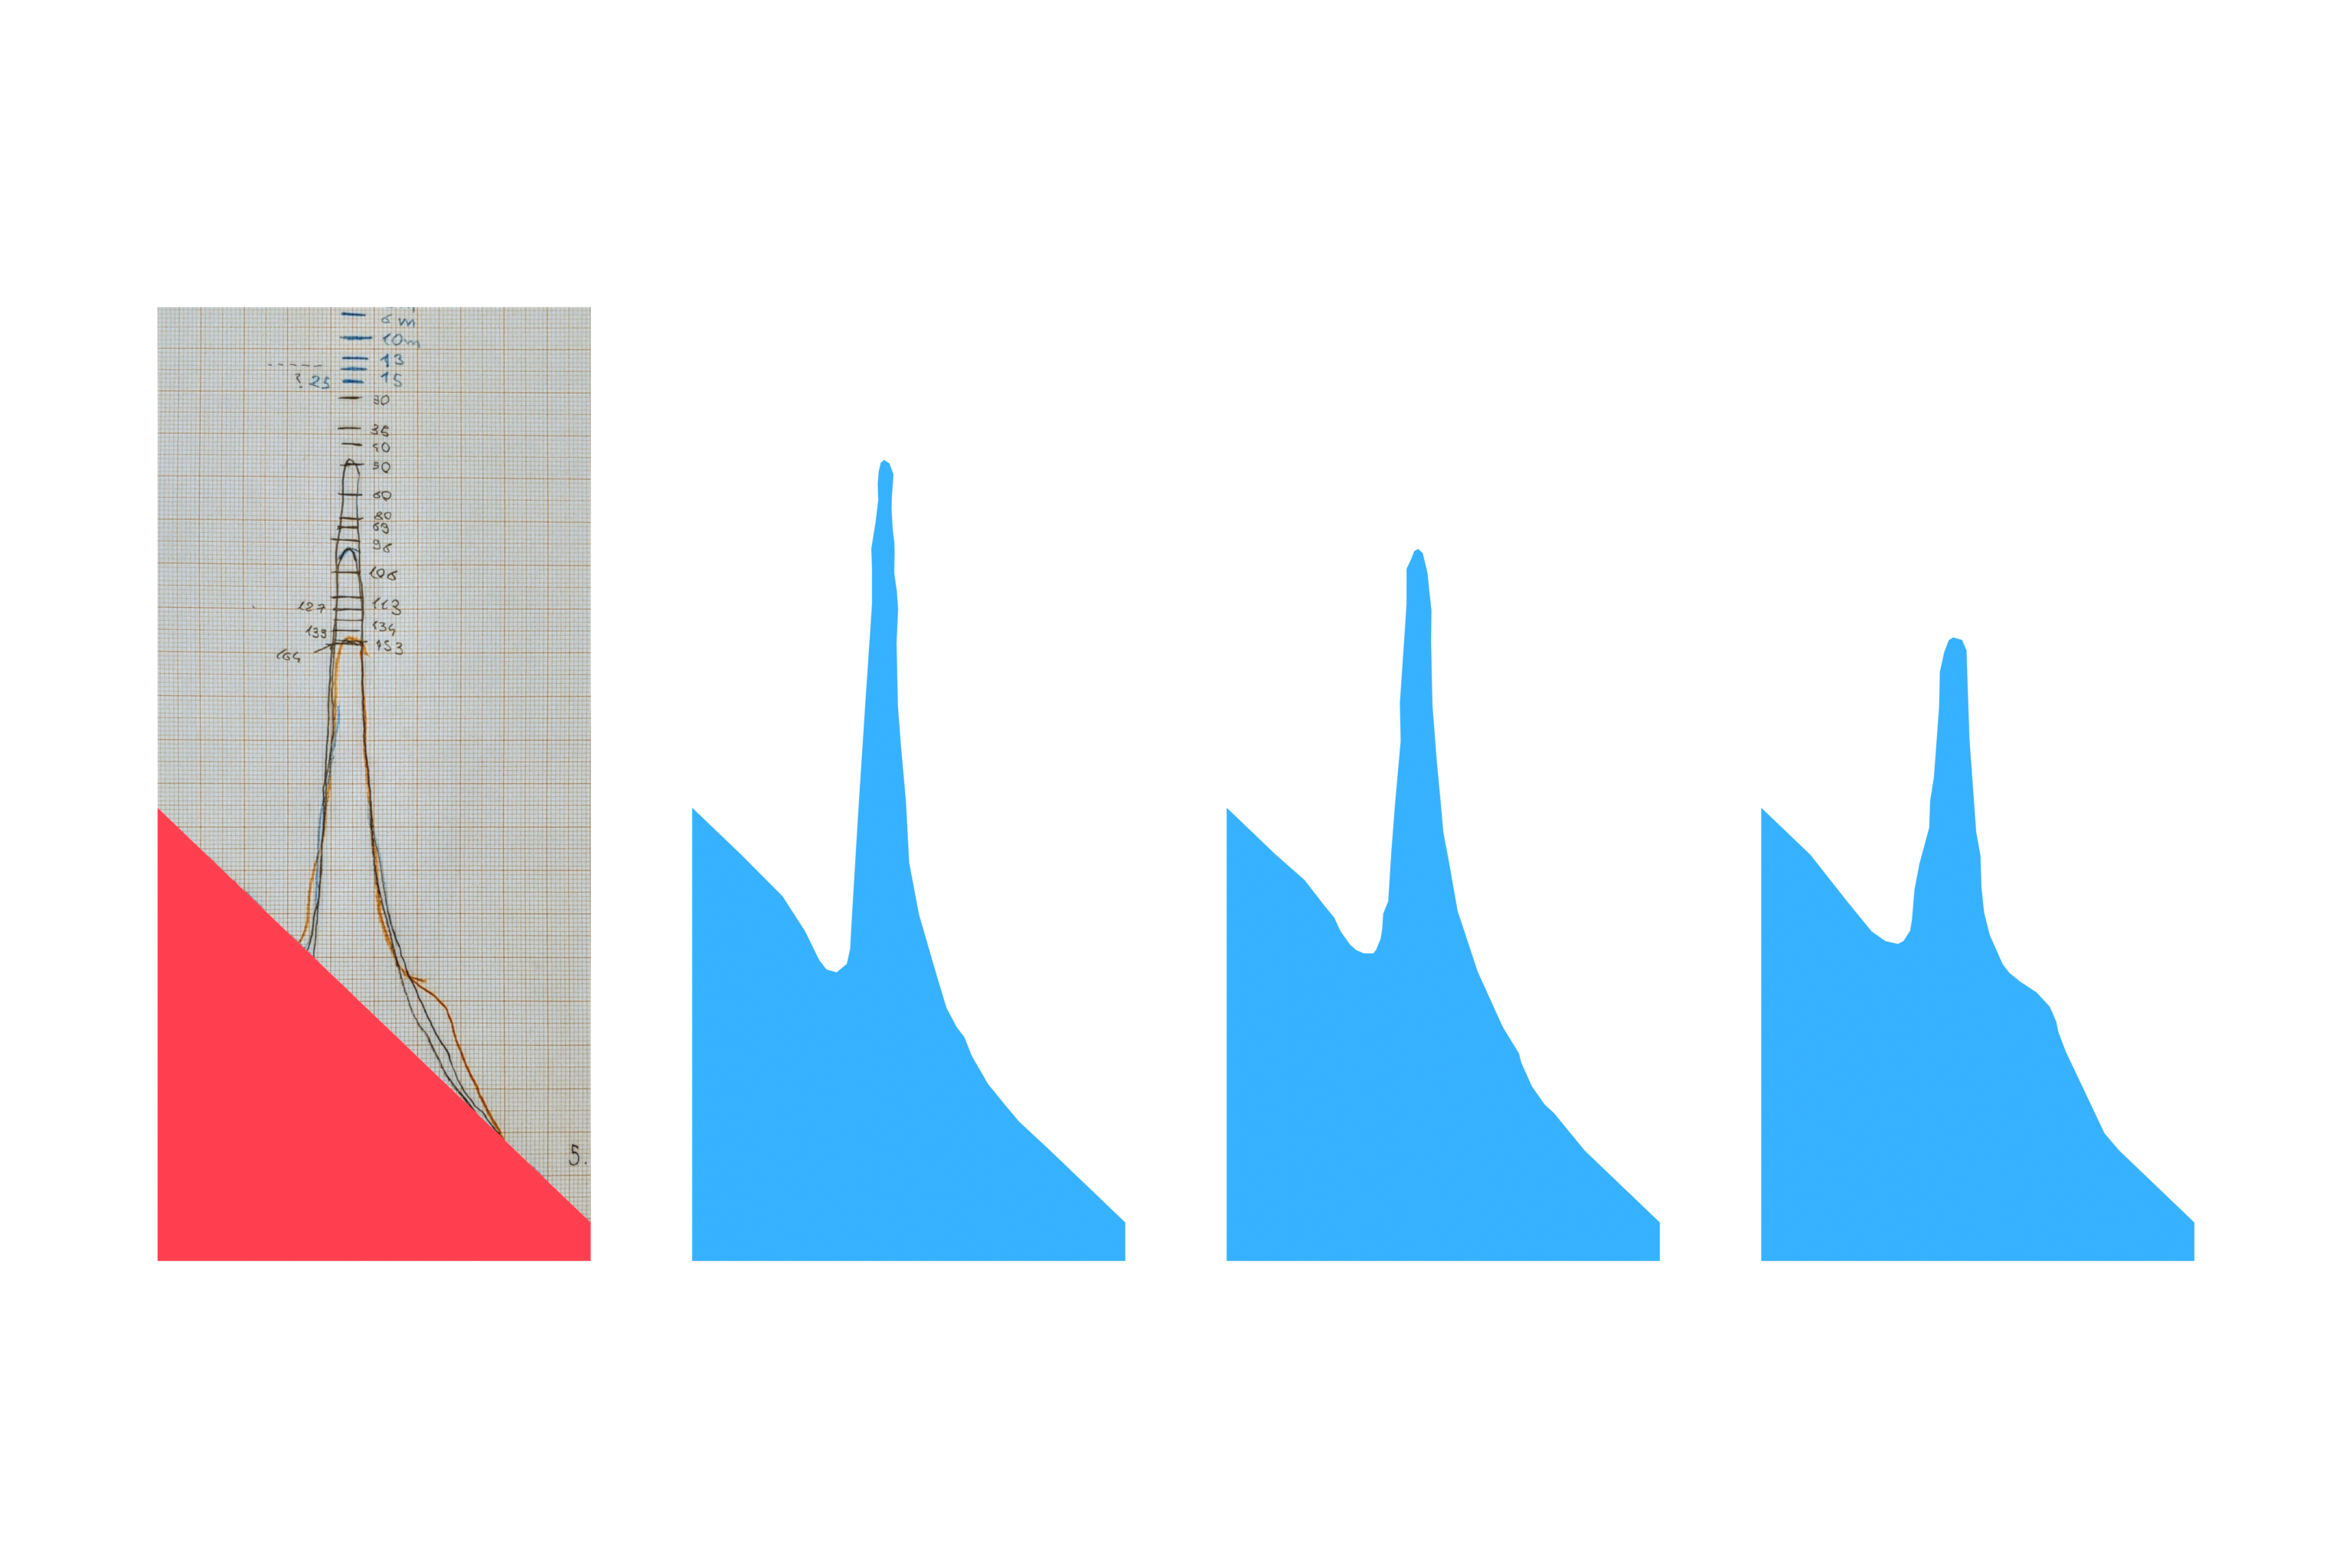
\includegraphics[width=\textwidth]{meas.png}
    \end{center}
    \caption{Krivulje, ki jih razberemo iz $10\times22\,\mathrm{cm}$ področja slike~\ref{fig:ticks}, orisane z n-kotnikom. Površino n-kotnika izračunamo tako, da seštejemo površino trikotnikov, ki ga sestavljajo. Z rdečo je narisana površina pod diagonalo, ki jo odštejemo modrim ploskvam, da dobimo površine $S_1$, $S_2$ in $S_3$.}
    \label{fig:meas}
\end{figure}

Iz enačbe~(\ref{eq:h}) lahko izrazimo časovno odvisen

\begin{equation*}
    Dt = \frac{1}{4\pi k^2} \left( \frac{S}{h} \right)^2.
\end{equation*}

Vse količine na desni strani izraza so znane iz meritev. Torej lahko na dano količino prilagodimo premico in kot njen naklon dobimo difuzijsko konstanto $D$ (slika~\ref{fig:linearized}). Izračunana vrednost konstante je

\begin{equation*}
    D = (1.86 \pm 0.07)\,\mathrm{m^2/s}.
\end{equation*}

\begin{figure}
    \begin{center}
        \includegraphics{linearized.pdf}
    \end{center}
    \caption{Meritve $\frac{1}{4\pi k^2} \left( \frac{S}{h} \right)^2$, ki so po izrazu~(\ref{eq:h}) preprosto premica z naklonom $D$.}
    \label{fig:linearized}
\end{figure}

\end{document}
